%!TEX root = ../../master.tex
\section{Host Operating System and Hypervisors}
\label{sec:role_of_os_and_hypervisors}
The operating system (OS) plays a different role in cloud computing than in traditional desktop computing. The physical machine and the OS becomes a simple resource in a shared pool of resources that is utilized by multiple tenants. Gartner defines multitenancy as:

\begin{definition} [Multitenancy \cite{gartner_multitenancy} ]
"Multitenancy is a reference to the mode of operation of software where multiple independent instances of one or multiple applications operate in a shared environment."
\end{definition}

\noindent
The OS in cloud computing must ensure isolation and multitenancy. According to Bernstein, primarily two technologies ensure this in cloud computing, namely hypervisors and containers \cite[p. 81]{bernstein2014containers}. 
A hypervisor, also called a Virtual Machine Monitor, is a layer on top of a host machine for running virtual machines. There are different types of hypervisors differentiating on whether or not there is an OS between the hypervisor and the host machine. 
\begin{itemize}
    \item \textbf{Type-1 native}: Hypervisors without an OS running on bare-metal
    \item \textbf{Type-2 hosted}: Hypervisors running on top of an OS (Figure \ref{fig:hypervisors_vs_containers})
\end{itemize}
\noindent
One of the early commercial type-1 hypervisors was VMware ESXi\footnote{https://www.vmware.com/products/esxi-and-esx/}, which is used for both private and public clouds. An example of a type-2 hypervisor is VMware Workstation\footnote{ http://searchvmware.techtarget.com/guides/VMware-Type-2-hypervisor-comparison-Workstation-vs-Player-vs-Fusion} that can run on a regular computer. The biggest player in cloud hosting, Amazon Web Services (AWS), use XEN Hypervisor\footnote{ www.xenproject.org}, and Microsoft uses their own Hyper-V for Microsoft Azure and their private cloud.
The benefits of using hypervisors are the isolation, dynamism, and the flexibility of running different operating systems. Among the drawbacks are the start-up time for the guest OS, and the size of each running instance. \\


\noindent
Containers share the host OS and eliminate the guest OS as seen in Figure \ref{fig:hypervisors_vs_containers}. This makes containers smaller to deploy than virtual machines. Furthermore, it is possible to run numerous containers on a single host. There have been several similar technologies through the time. Bernstein summarizes the inspiration as being the Unix command \textit{chroot} from 1979, \textit{jail} in FreeBSD from 1998, and \textit{zones} in Solaris 10 from 2004. In 2006, Google contributed \textit{cgroups} to the Linux kernel. Google has used containers for their internal services since 2004. As of 2014 Google deployed over two billion containers per week and over 3000 per second \cite{sanchez2014google_containers}. Burns et al describe one of Google's motivations for using containers: \textit{"The resource isolation provided by containers has enabled Google to drive utilization significantly higher than industry norms"} \cite[p. 4]{burns2016borg_omega_kubernetes}. \\

\noindent
In 2008 Linux Containers (LXC) were created which layered a more user-friendly tooling around \textit{cgroups} and \textit{namespaces}. However, containers were not popularized until Docker in 2013 provided an even more user-friendly interface for LXC.

\begin{figure}[H]
    \centering
    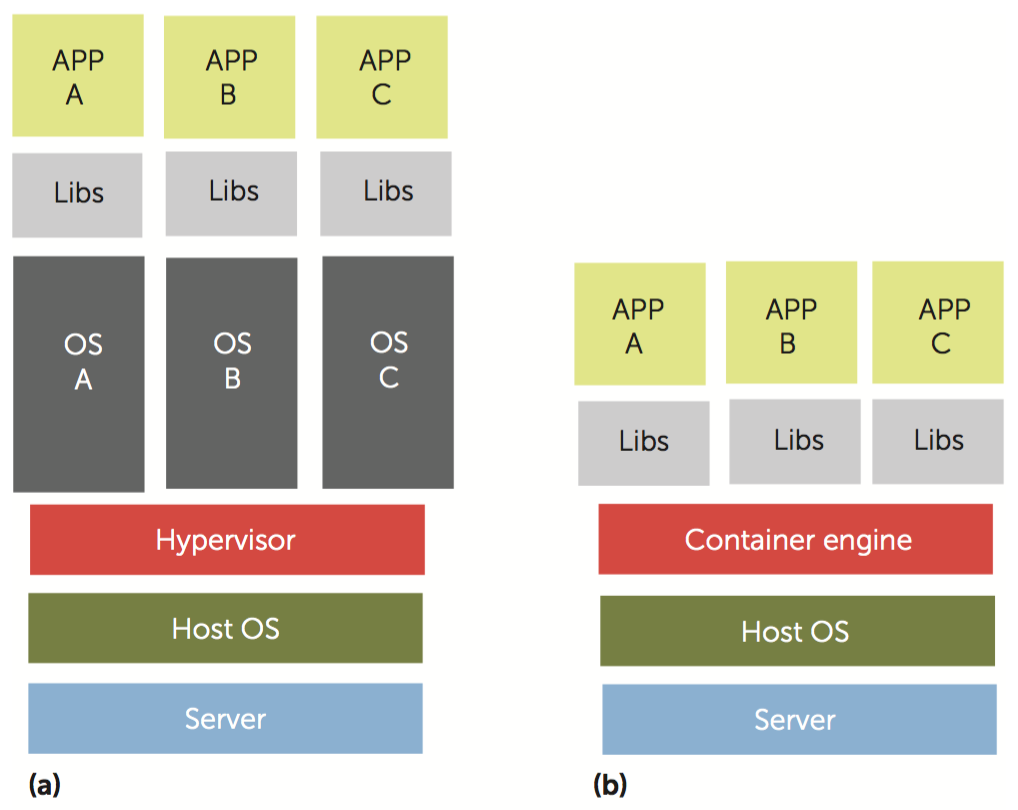
\includegraphics[scale=0.6]{figures/hypervisor_vs_container}
    \caption{Hypervisors (type 2) and Containers \cite[p. 82]{bernstein2014containers}}
\end{figure}
\label{fig:hypervisors_vs_containers}

\noindent
In summary, the difference between hypervisors and containers is that virtual machines on hypervisors run an entire OS whereas containers extend a running kernel. According to Joy's performance comparison between Linux Containers and virtual machines, \textit{"containers have outperformed virtual machines in terms of performance and scalability", and continues "because of its better scalability and resource utilization, containers can be used for application deployments to reduce resource overhead."} \cite[p. 346]{joy2015performance}.
%%%%%%%%%%%%% HERTIL

%\section{Containers}
%\label{sec:cloud_containers}
%Containers share the host OS and eliminate the guest OS as seen en figure \ref{fig:hypervisors_vs_containers}. This makes containers smaller to deploy and makes it is possible to store hundreds of containers on a single host. There has been several similar technologies through the time. Bernstein summarizes the inspiration as being the Unix command \textit{chroot} from 1979, \textit{jail} in FreeBSD from 1998, \textit{zones} in Solaris 10 from 2004, and other Unix vendors in the time after that. In 2006 Google released \textit{cgroups} for the Linux kernel, and Google has used containers for their services since 2004. As of 2014 Google deployed over two billion containers per week and over 3000 per second\footnote{ http://www.infoq.com/news/2014/06/everything-google-containers}. In 2008 Linux Containers (LXC) were created which layered a more user friendly tooling around \textit{cgroups} and \textit{namespaces}\footnote{ http://rhelblog.redhat.com/2015/08/28/the-history-of-containers/}.
%\\ \\
%Bernstein mentions Google among other successful cloud platforms in 2014, and since then both Amazon and Microsoft have added a container service to their portfolio.
\subsection*{Docker}
In 2013, the container project \textit{Docker} was released. Docker is an API on top of Linux Containers (LXC) that has gained a lot of popularity. Bernstein explains Docker as: \textit{"Docker extends LXC with a kernel- and application-level API that together run processes in isolation"} \cite[p. 82]{bernstein2014containers}. Docker helps standardize working with containers by providing a uniform interface. The two main concepts of Docker are containers and images. A container is the name of a running instance that is constructed from an image. Images are either downloaded from a registry, build manually, or a combination starting from an image and extending with additional layers. Images are like LEGO bricks. They can be stacked on top of each other (Figure~\ref{fig:docker_image}). A Docker image contains an application and its needed dependencies, which includes the runtime environment. The layers in a Docker image are filesystem layers as seen in Figure \ref{fig:docker_image}. Docker provides a declarative definition of an environment (Dockerfile) which ensures that an application always runs in the same environment. Docker removes the need to maintain and worry about different versions of languages and runtimes on servers since it is contained in the image. Docker eliminates the classic problem of differences in the developer and production environment. Turnbull explains this problem between developers and operations as: \textit{"It works on my machine; it's operations' problem now"} \cite[p. 103]{anderson2015docker}.

\begin{figure}[H]
    \centering
    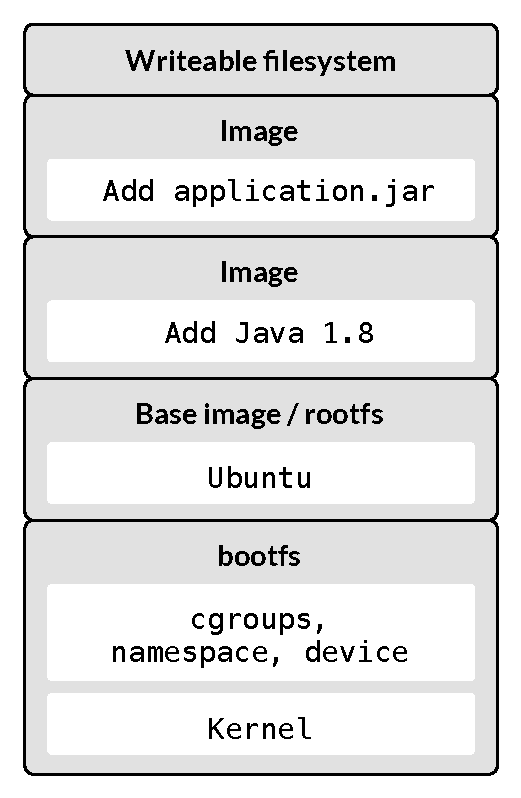
\includegraphics[width=4.5cm]{figures/docker_image}
    \caption{Docker Image Layering}
    \label{fig:docker_image}
\end{figure}

\noindent
Turnbull further describes the layered filesystem in Docker as 
\cite[p. 2-3]{turnbull2016dockerbook}, the bottom layer consists of typical Linux boot filesystems called \textit{bootfs} which is mounted in a read-only mode. When the boot has finished, the container (notice the transition from image to container) is moved into memory, and the boot filesystem is unmounted. The next layer is a root filesystem called \textit{rootfs} which can be different base images such as Debian or Ubuntu. This layer is also referred to as the base image. Rootfs is mounted and stays in read-only mode unlike a traditional Linux boot, where the mode is changed to read-write after successful boot. This is made possible by \textit{union mount} which is a way of combining multiple filesystems while maintaining the view of a single filesystem. Files and directories are, in other words, added on top of each other. In this way, several read-only layers are combined, and on top, a writeable layer is added. This permits changes in the container while sharing images between containers since modifications are kept in a small writeable layer on the top. Images are stacked on top of parents as seen in Figure \ref{fig:docker_image}. \\


\noindent
Docker consists of a command line client and a daemon running on a host machine. The daemon runs on a Linux machine but the client can run on Linux, Windows and OS X. The communication between client and daemon can either be a TCP connection or a Unix socket which makes it possible to point clients to different daemons. Docker's architecture\footnote{\url{https://docs.docker.com/engine/understanding-docker/}} is depicted in Figure~\ref{fig:docker_architecture}.

\begin{figure}[H]
    \centering
    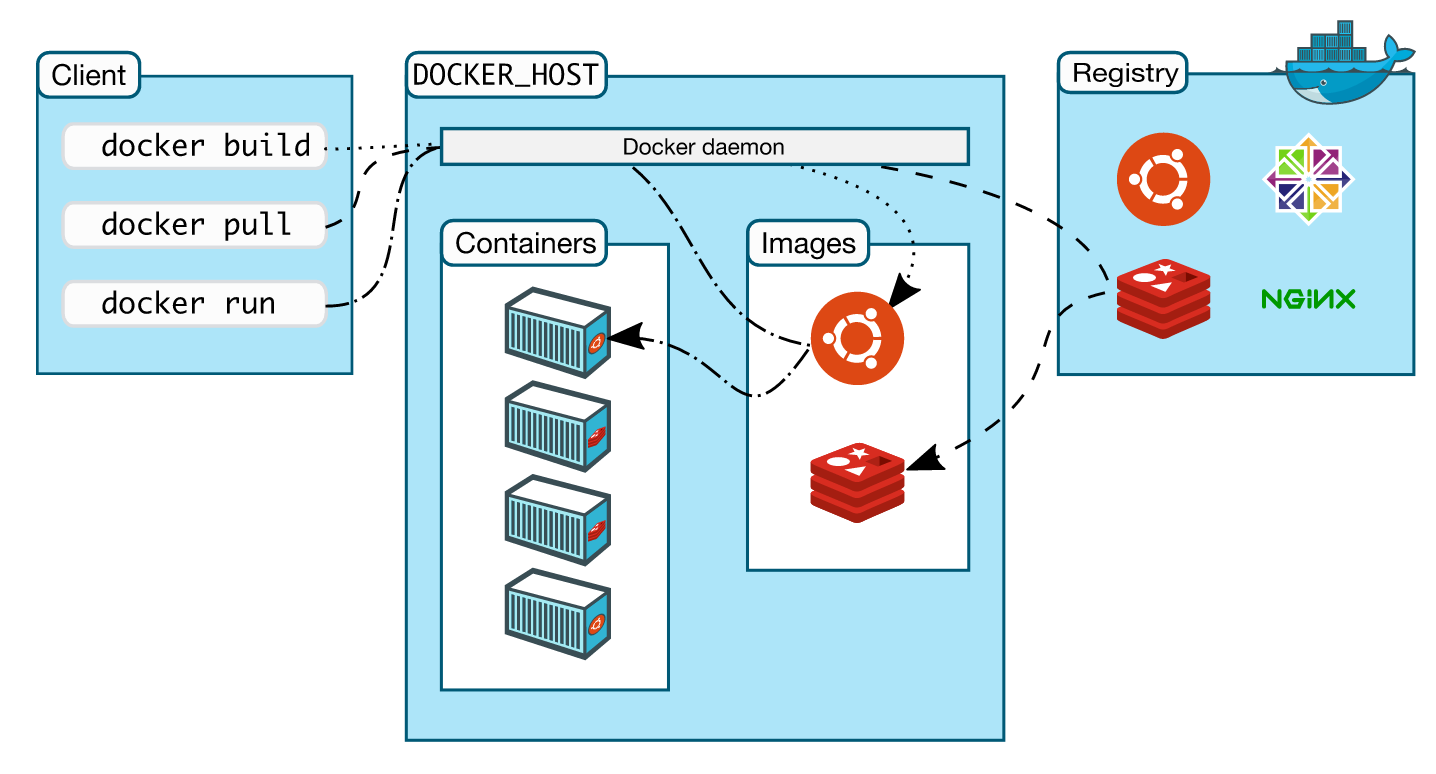
\includegraphics[scale=0.45]{figures/docker_architecture}
    \caption{Docker Architecture}
    \label{fig:docker_architecture}
\end{figure}


\noindent
Registries, such as Docker Hub\footnote{\url{https://hub.docker.com/}}, contain images with prepared environments. This enables diverse environments and changes without having to install and maintain different runtime versions on different servers. Images can be pulled and pushed similar to Git. Because of the layering, only the difference is pulled or pushed, which is the new layer(s). One thing to keep in mind, when using other's images, is whether or not they contain security issues. \\

\noindent
The challenges of management, scheduling, and service discovery arise when moving from one container to multiple containers that communicate with each other. These challenges will be described in the following section.

\section{Cluster Management}\label{sec:cluster_management}
A cluster can be viewed as an abstraction comprised of multiple machines (virtual or physical). Combined, the machines (nodes) form a resource pool that can be viewed as a single entity e.g. three machines (Figure~\ref{fig:cloud_abstraction}) with 2 CPU cores and 8GB RAM would have the total compute power of 6 cores and 24GB RAM. Machines in cloud computing are degraded to a simple utility. Bill Baker, Distinguished Engineer at Microsoft, describes this shift with an analogy of treating servers like cattle instead of pets. 

\begin{figure}[H]
    \centering
    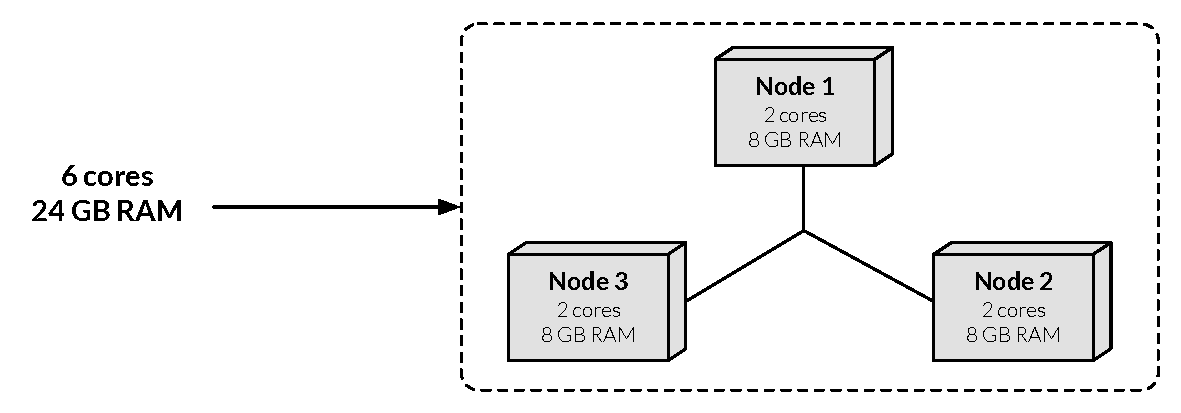
\includegraphics[width=13cm]{cloud_abstraction}
    \caption{Cloud Abstraction}
    \label{fig:cloud_abstraction}
\end{figure}

\noindent
The view of machines as simple, homogeneous resources allows for a more dynamic environment. The dynamic environment makes it easier to scale the number of running instances (e.g. containers) to the current load. Taking care of resource allocation in an intelligent way while dynamically connecting instances becomes a complex task. Furthermore, the paradigm shift towards service-oriented architectures makes it even harder to orchestrate the increasing amount of services. This leaves an immense task on cluster management systems to orchestrate instances of services. These tasks include creating an appropriate cluster abstraction of multiple machines, optimizing resource scheduling, keeping services running and to some degree sustaining resilience. \\

\subsection*{The Bin Packing Problem}
Kelsey Hightower, Staff Developer Advocate from Google, explains\footnote{\url{https://www.youtube.com/watch?v=9v8LReolgZ8}} the challenge of resource scheduling optimization as \textit{the bin packing problem}. The concern of the bin packing problem is to pack workloads of different sizes into a finite amount of bins (nodes) while minimizing the number of bins. In other words, optimizing the utilization of resources in terms of e.g. CPU and memory within each bin without increasing the amount of bins as the only solution. Scheduling applications in an intelligent way can avoid resource waste but the bin packing problem is classified as having an NP-hard computational complexity. If an application requires a lot of CPU and only little memory then there is a risk of blocking memory resources for other applications (Figure~\ref{fig:bin_packing} - node b).

\begin{figure}[H]
    \centering
    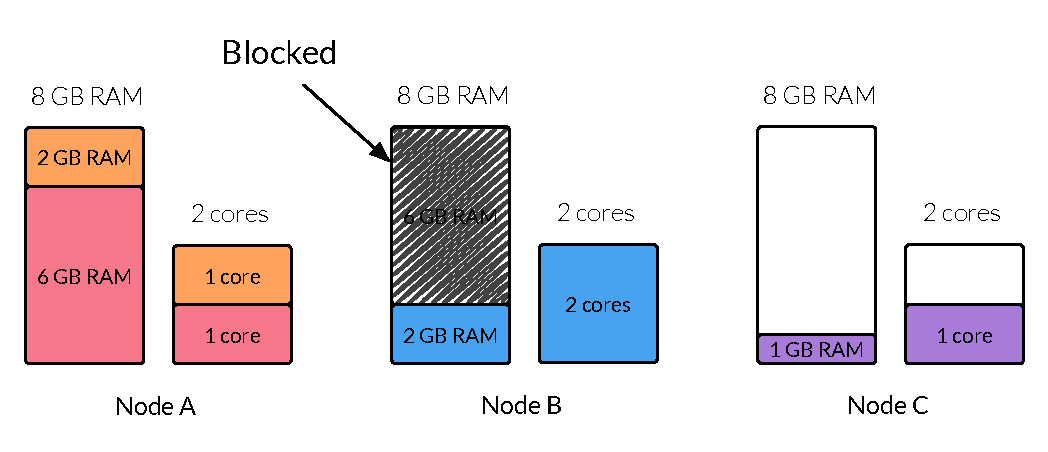
\includegraphics[width=12cm]{bin_packing}
    \caption{The Bin Packing Problem}
    \label{fig:bin_packing}
\end{figure}

\noindent There exist many cluster management systems created by big web-scale companies. We will in the following discuss Docker Swarm, Apache Mesos, and Kubernetes.

\subsection*{Docker Swarm}
Docker Swarm is an abstraction on top of Docker. Docker Swarm utilizes the standard Docker API, but instead of running all containers on the same Docker host they are distributed across a swarm of Docker hosts. For scheduling the containers across different hosts, a Swarm manager is introduced. The rest of the hosts run Swarm agents that communicate with the manager. The strategies for scheduling containers are: spread, BinPack and random. Spread favors a low amount of containers on each node while BinPack favors packing according to the memory usage. Furthermore, Docker Swarm can create replica instances across a cluster. The first non-beta version of Swarm was released in September 2015, which makes it a relatively new option.

\subsection*{Apache Mesos}
Apache Mesos, on the other hand, is a well-tested option that Twitter has used and contributed to since 2010, and currently a lot of successful cloud companies such as Netflix, Airbnb, and Uber use Mesos\footnote{http://mesos.apache.org/documentation/latest/powered-by-mesos/}. Mesos is designed with high-availability and resilience in mind \cite{mouat2015orchestration_tools}. Mesos is described as a distributed systems kernel that can be used to schedule many different types of workloads. \textit{Mesos Agent Nodes} do the work and report their free resource to a \textit{Mesos Master}. A \textit{Mesos Master} sends tasks to Agents and offers resources to \textit{Frameworks} according to an allocation strategy. \textit{Frameworks} consist of an executor process on each Agent to handle the execution. The Mesos architecture is depicted in Figure~\ref{fig:mesos_architecture}.

\begin{figure}[H]
    \centering
    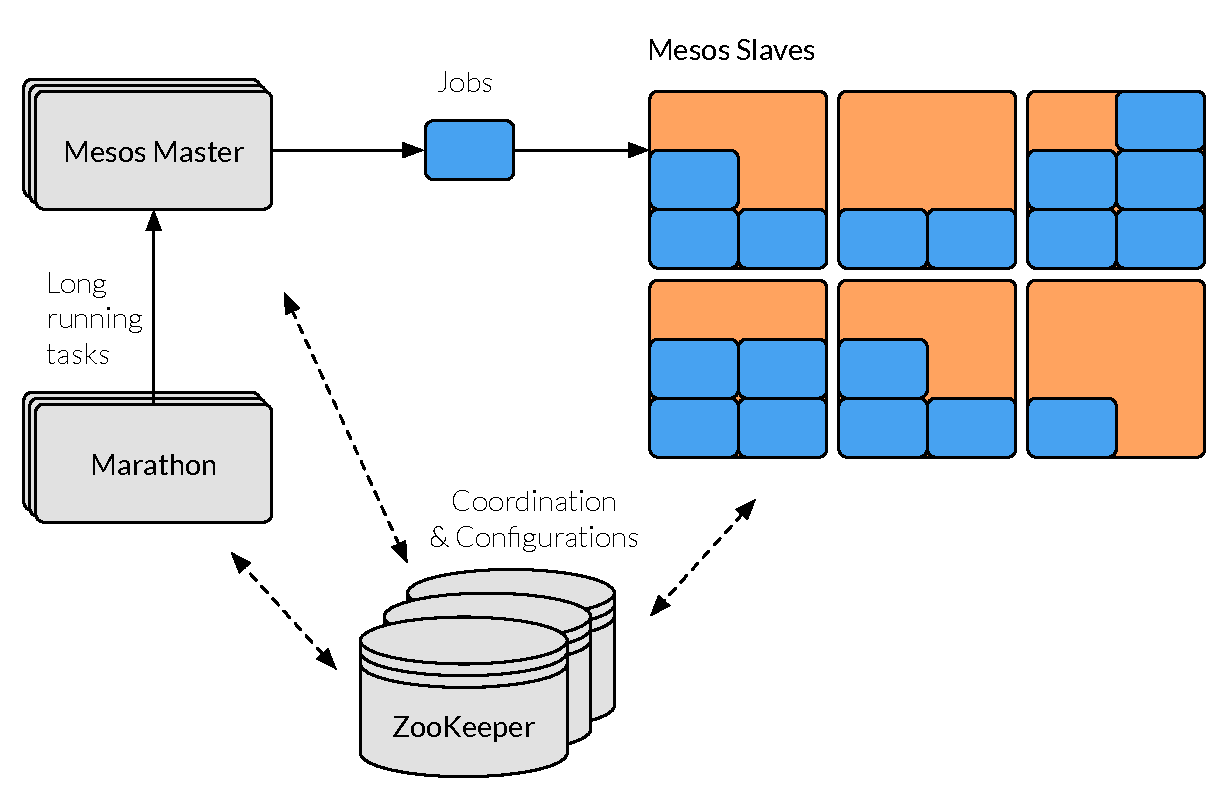
\includegraphics[width=12cm]{figures/mesos_architecture}
    \caption{Mesos Architecture}
    \label{fig:mesos_architecture}
\end{figure}

\noindent
Since Mesos is designed for resilience, the master is replicated with an elector, called \textit{ZooKeeper}, in front of it. \textit{ZooKeeper} makes sure that agents can find the master, and the ZooKeeper itself is also usually replicated. Marathon is a container orchestration platform that runs on top of Mesos. 

\subsection*{Kubernetes}
Google is a pioneer in container technology. Burns describes: \textit{"Containerization transforms the data center from being machine-oriented to being application-oriented"} \cite[p. 74]{burns2016borg_omega_kubernetes}. Google's internal container management platform, called Borg \cite{verma2015borg}, takes care of the challenges involved running web-scale cluster management. In 2014, Google announced and released an open source cluster management system called Kubernetes that is similar to Borg. Kubernetes builds upon many of the concepts in Borg and is \textit{"an open-source platform for automating deployment, scaling, and operations of application containers across clusters of hosts, providing container-centric infrastructure"} \cite{kubernetesio}. Kubernetes is chosen for KubeCloud. The choice will be discussed in Chapter~\ref{chap:tangible_cluster}. A high-level overview of Kubernetes is depicted in Figure~\ref{fig:kubernetes_architecture_report}.

\begin{figure}[H]
    \centering
    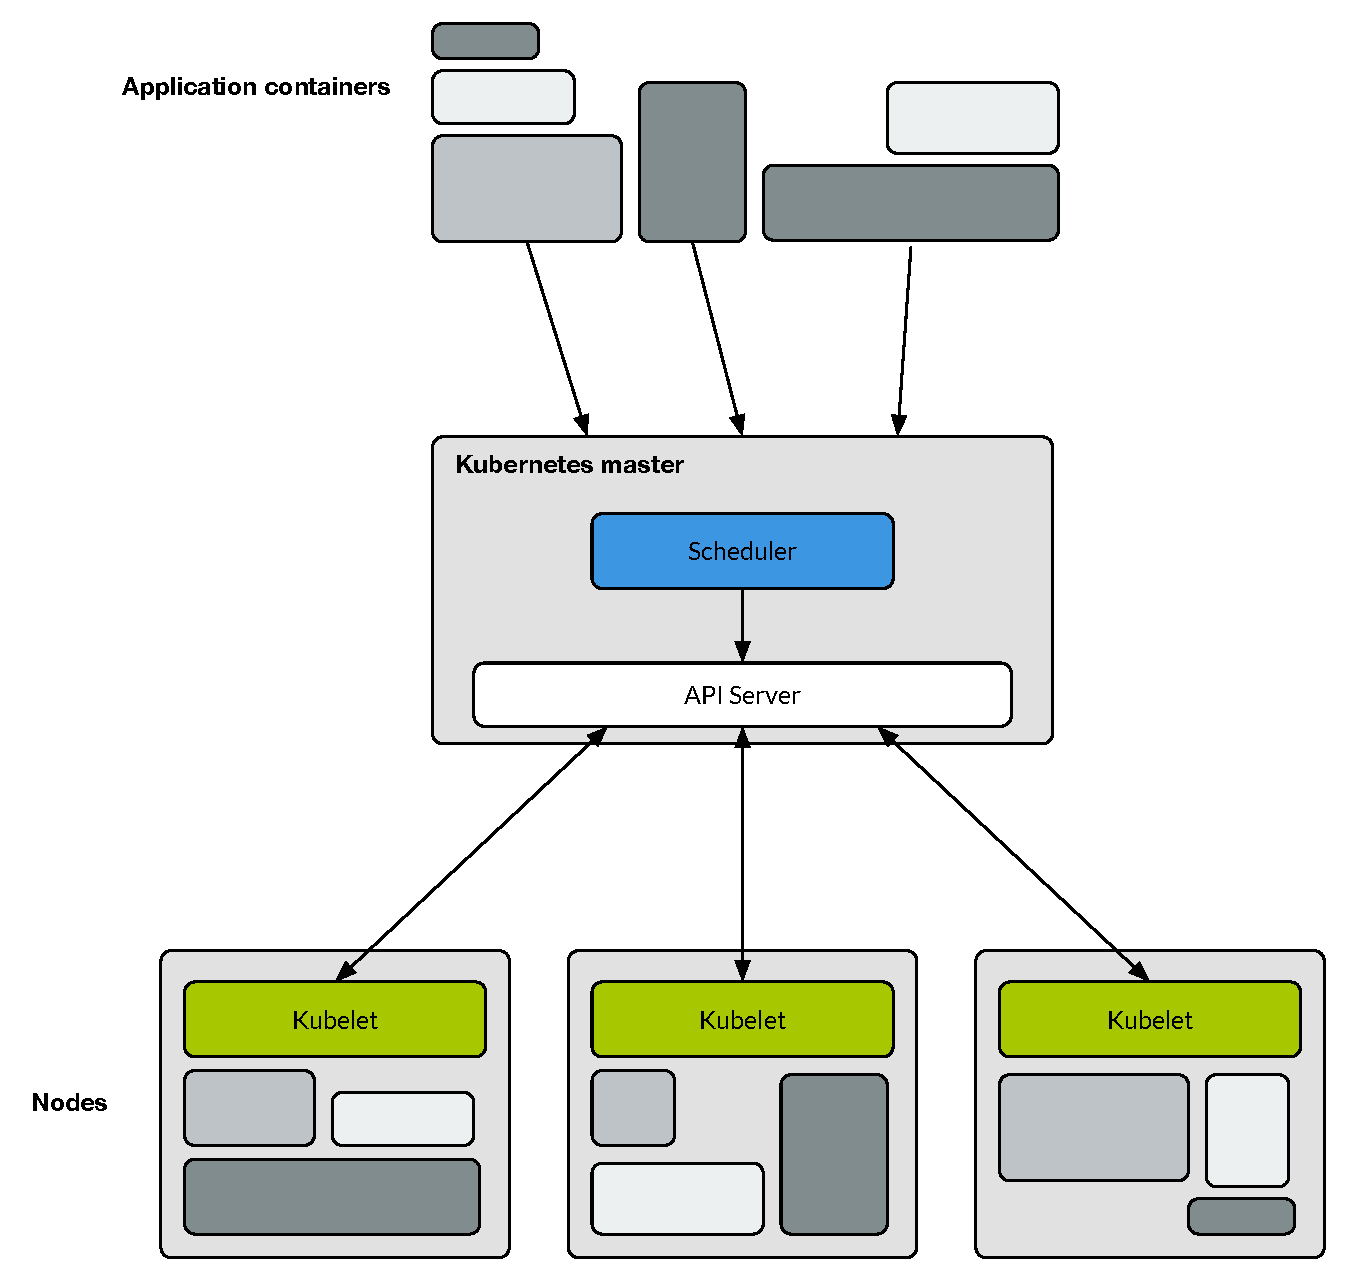
\includegraphics[width=12cm]{figures/kubernetes/architecture}
    \caption{Kubernetes Architecture}
    \label{fig:kubernetes_architecture_report}
\end{figure}

\noindent
From a high-level perspective, we see three main parts in the Kubernetes workflow. First, we have the application containers or the workload that Kubernetes needs to handle. Next, we have the Kubernetes master, who is in charge of scheduling the workload, communicating with the workers (nodes), keeping track of the cluster, etc. Lastly, the workers consume the workloads and execute given tasks. \\
%% Master/worker


\noindent
The Kubernetes master is the controlling unit in Kubernetes. It serves as the main management contact point for administrators, and it provides a range of cluster-wide services for the Kubernetes workers. Figure~\ref{fig:kubernetes_master_report} shows an overview of the main components of the Kubernetes master deployed on a single node. 

\begin{figure}[H]
    \centering
    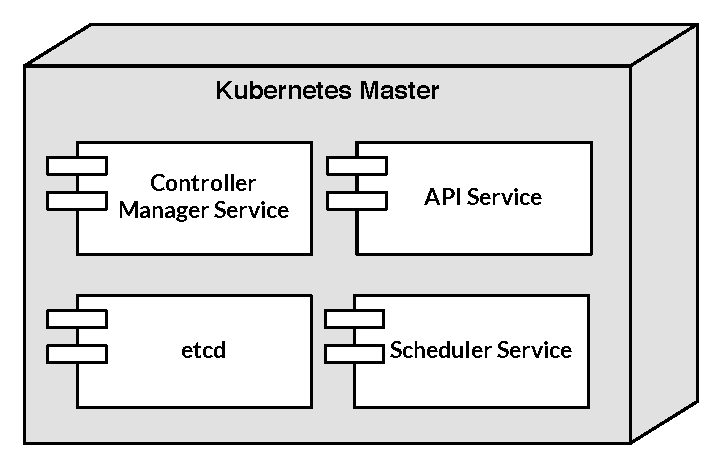
\includegraphics[width=8cm]{figures/kubernetes/kubernetes_master}
    \caption{Kubernetes Master}
    \label{fig:kubernetes_master_report}
\end{figure}

\noindent Figure~\ref{fig:kubernetes_master_report} displays the four main components involved in the responsibilities of the Kubernetes master. 

\subsubsection*{etcd}
In Kubernetes, etcd is a fundamental component. It is a globally available configuration store developed by CoreOS. Ellingwood defines etcd as: \textit{"etcd is a lightweight, distributed key-value store that can be distributed across multiple nodes"} \cite[p. 3]{digitalocean2014kubernetes}. Kubernetes stores configuration data in etcd. This data is accessed by the nodes and can be used for service discovery. Furthermore, the etcd store represents the state of each node and the cluster in its entirety.


\subsubsection*{Controller Manager Service}
The Controller Manager Service handles the replication processes used in Kubernetes defined by the Replica Sets (introduced later). The controller manager uses etcd to write the details of these operations. Furthermore, the controller manager watches for changes in etcd. Ellingwood describes this concept as: \textit{"When a change is seen, the controller manager reads the new information and implements the replication procedure that fulfills the desired state"} \cite[p. 4]{digitalocean2014kubernetes}.



\subsubsection*{API Service}
The API service is the main management point of the entire cluster. The API service allows users to deploy applications and control many of the Kubernetes workloads and configurations. Furthermore, the API service is responsible for aligning the etcd store with the service details of the deployed containers. The API service is implemented as a RESTful interface, which allows ease of communication for different tools and libraries.


\subsubsection*{Scheduler Service}
The scheduler is responsible for assigning workloads to specific nodes. The scheduler determines which node to deploy a workload on by reading the workload's operating requirements, analyzes the current infrastructure environment, and then places the work on the node best fit for the workload.

\subsubsection*{Add-On Services}
Kubernetes' architecture is loosely coupled and allows for easy add-on of additional services. 
\begin{itemize}
  \item \textbf{Heapster:} Heapster enables Container Cluster Monitoring and Performance analysis (cAdvisor aggregation).
  \item \textbf{KubeDNS / SkyDNS}: DNS service for resolving services instead of using IPs directly.
  \item \textbf{Registry}: Local Container Registry instead for depending on Docker Hub. 
\end{itemize}


\noindent
The Kubernetes worker performs the work in the cluster. Kubernetes workers have few requirements necessary to communicate with the Kubernetes master. Furthermore, the container network has to be configured in order for the worker to be able to run the workloads assigned to them. Figure~\ref{fig:kubernetes_slave_report} shows the deployment diagram of a Kubernetes worker and the components it is comprised of.

\begin{figure}[H]
    \centering
    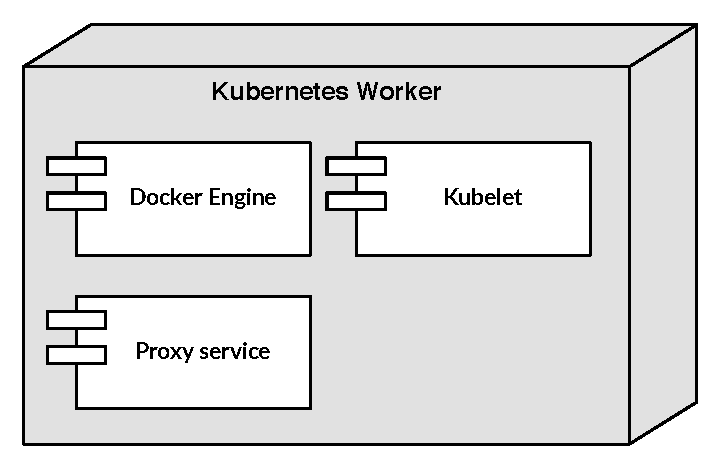
\includegraphics[width=8cm]{figures/kubernetes/kubenetes_slave}
    \caption{Kubernetes Worker}
    \label{fig:kubernetes_slave_report}
\end{figure}

\noindent The Kubernetes worker consist of three main components as visualized in Figure~\ref{fig:kubernetes_slave_report}. These three components will be described below.

\subsubsection*{Docker Engine}
Since Kubernetes runs and manages containers, specifically Docker containers (other container formats can be used as well), Docker has to run on each worker. Docker is used to run the containers of the specific hosts that they are being scheduled to. Kubernetes makes the key assumption that each node has a dedicated subnet available to the Docker engine in order for pods to communicate. Different approaches can be used to fulfil this requirement. The approach in KubeCloud will be discussed in Chapter~\ref{chap:tangible_cluster}.

\subsubsection*{Kubelet}
The Kubelet is a small service that acts as the main contact point for the Kubernetes worker with the Kubernetes master. Ellingwood describes the Kubelet's responsibility as: \textit{"This service is responsible for relaying information to and from the master server, as well as interacting with the etcd store to read configuration details or write new values"} \cite[p. 5]{digitalocean2014kubernetes}.


\subsubsection*{Proxy Service}
The proxy service is responsible for dealing with the host subnetting and making services available by forwarding request to the correct containers. The general responsibility of the proxy service can be summarized to making sure the networking environment is predictable and accessible, but still isolated.
%%


\subsubsection*{Lessons Learned in Running Borg}
Verma et al (Google) describe their lessons learned with Borg, \textit{"We've learned from operating Borg in production for more than a decade, and describe how these observations have been leveraged in designing Kubernetes"} \cite[p. 13]{verma2015borg}, as:

\begin{itemize}
    \item \textbf{The good:} 
        \begin{itemize}
            \setlength\itemsep{0.05em}
            \vspace{-3mm}
            \item Allocs are useful
            \item Cluster management is more than task management
            \item Introspection is vital
            \item The master is the kernel of a distributed system
        \end{itemize}
    \item \textbf{The bad:} 
        \begin{itemize}
            \setlength\itemsep{0.05em}
            \vspace{-3mm}
            \item Jobs are restrictive as the only grouping mechanism for tasks
            \item One IP address per machine complicates things
        \end{itemize}
\end{itemize} 

\noindent
The first good lesson learned in running Borg is that \textbf{Allocs are useful}: \textit{"A Borg alloc is a reserved set of resources on a machine in which one or more tasks can be run"} \cite[p. 3]{verma2015borg}. In Kubernetes, an alloc is equal to a \textit{pod}. A pod is the central unit that Kubernetes schedules, and a pod consists of a group of one or more containers e.g. Docker containers). This means that Docker containers themselves are not assigned to a host, instead they are nested inside another container, called a pod. A pod can contain one or more containers, and cohesive containers are usually deployed together in a single pod. When containers are deployed together inside a pod, they can leverage a shared IP address and port space, and communication via localhost is possible. Effective container-to-container communication is, thereby, a solved problem. This is the first of four identified network problems that Kubernetes solves \footnote{\url{http://kubernetes.io/docs/admin/networking/}}. Figure~\ref{fig:pods_report} shows two scenarios; (left) a single container deployed in a pod, (right) two containers deployed in the same pod.

\begin{figure}[H]
    \centering
    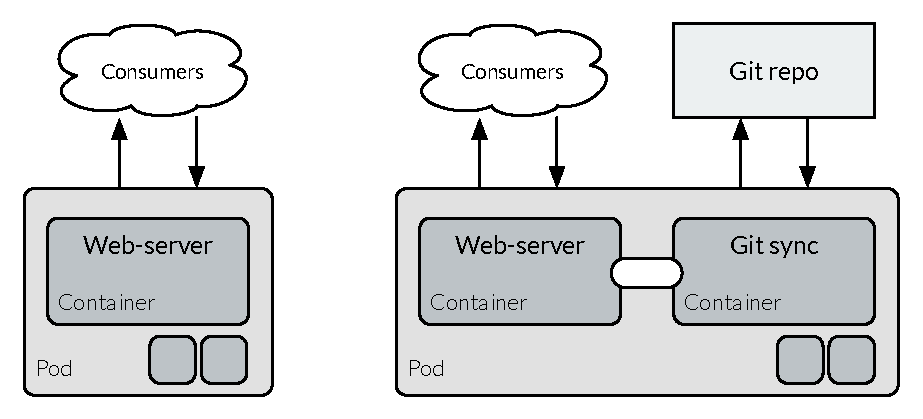
\includegraphics[width=12cm]{figures/kubernetes/pods}
    \caption{Pods}
    \label{fig:pods_report}
\end{figure}

\noindent
The figure on the right in Figure~\ref{fig:pods_report} shows two applications running in the same pod. The example contains a worker application fetching configurations from a Git repository and streams it to a web-server. The communication between these two containers could be over localhost. A pod is always scheduled on the same host, meaning a pod cannot span multiple hosts. Different pods can be located on different machines, and pod-to-pod communication over a network (networking problem number two) is thereby necessary. Pod-to-pod communication is achieved by leveraging that each pod has an IP address in a flat, shared networking namespace. The IP is either assigned by a cloud provider or a software defined network. In this way, all pods can communicate with each other, and conflicting port allocation among pods on the same host is not a problem.
 \\



\noindent
The second good lesson learned in running Borg is \textbf{Cluster management is more than task management}. \textit{"The applications that run on Borg benefit from many other cluster services, including naming and load balancing"} \cite[p. 14]{verma2015borg}. In Kubernetes, naming and load balancing is supported using the \textit{service} abstraction. A service acts as a load balancer in front of replicated pods. The definition of a service is: \textit{"A Kubernetes Service is an abstraction which defines a logical set of Pods and a policy by which to access them - sometimes called a micro-service"} \cite{kubernetesio}. Pods are targeted using a label selector, as visualized in Figure~\ref{fig:services_report}. The label selector in Figure~\ref{fig:services_report} is type=FE. This results in all pods having this label will receive traffic from the service.

\begin{figure}[H]
    \centering
    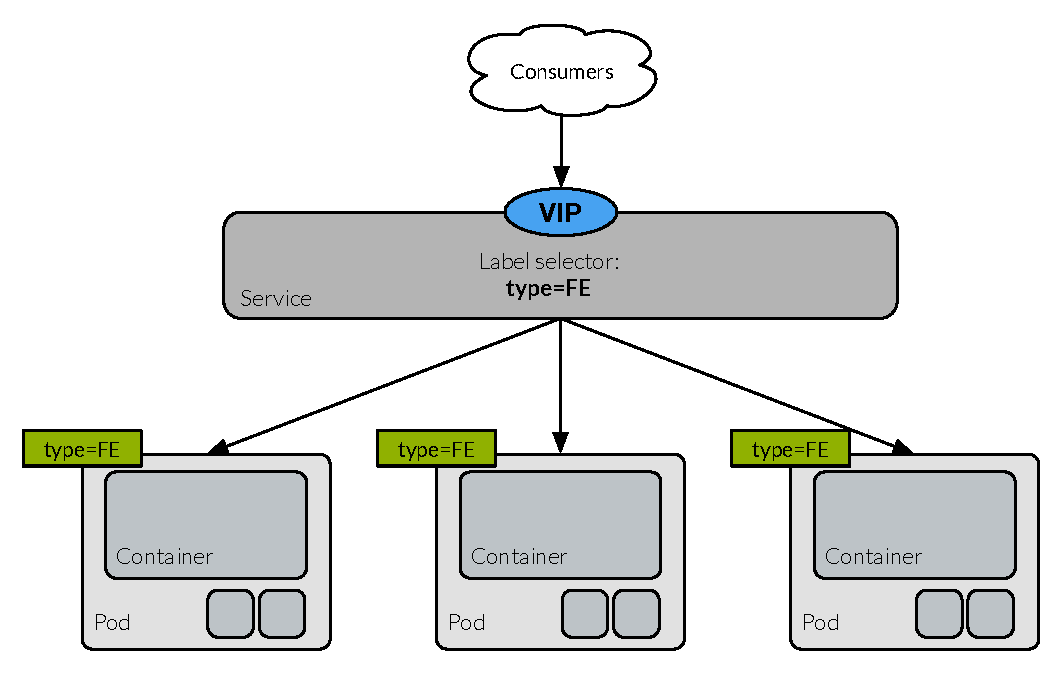
\includegraphics[width=14cm]{figures/kubernetes/service}
    \caption{Services}
    \label{fig:services_report}
\end{figure}

\noindent 
Services are assigned a static Virtual IP (VIP) in the range of service IPs defined in the Kubernetes API server. Opposite pods, services will keep the IP throughout its lifetime whereas pods dynamically can be started and killed. Services solve the third networking problem of pod-to-service communication by using the Virtual IP that transparently proxies to pods. Furthermore, services solve the fourth networking problem of external-to-service communication. Cloud providers can integrate load balancers with services, but solutions using the proxy service in the workers also exist. \\

\noindent
The third good lesson learned in running Borg is \textbf{Introspection is vital}. \textit{"An important design decision in Borg was to surface debugging information to all users rather than hiding it"} \cite[p. 14]{verma2015borg}. Kubernetes includes some of Borg's introspection techniques such as the resource monitoring tool, cAdvisor. cAdvisor allows for individual monitoring of a node's resources e.g. CPU and memory. \\

\noindent
The last good lesson learned in running Borg is \textbf{The master is the kernel of a distributed system}. \textit{"Borg was originally designed as a monolithic application"} \cite[p. 14]{verma2015borg}, but over time some parts of Borg (e.g. the scheduler) was split into services in order to scale up the workload and feature set. Kubernetes was designed as composable microservices from the beginning. All Kubernetes' microservices are clients of the API server (Figure~\ref{fig:kubernetes_master_report} and Figure~\ref{fig:kubernetes_slave_report}). \\ 

\noindent
The first bad lesson learned in running Borg is \textbf{Jobs are restrictive as the only grouping mechanism for tasks}. \textit{"Borg has no first-class way to manage an entire multi-job service as a single entity, or refer to related instances of a service"} \cite[p. 14]{verma2015borg}. Users of Borg hacked their way around this by encoding their service topology in the job name. To avoid these workarounds, Kubernetes instead organizes its pods using labels. \textit{"Labels are key/value pairs that are attached to objects such as pods"} \cite{kubernetesio}. Kubernetes connects objects together with labels and can be viewed as a grouping mechanism. The use of labels reduces coupling. Furthermore, labels can be added or removed during the lifecycle of the object. An example of labels used as meta-data for a pod can be seen in Figure~\ref{fig:labels_report}. A further example of labels is shown in Appendix~\ref{appendix:kubernetes}.

\begin{figure}[H]
    \centering
    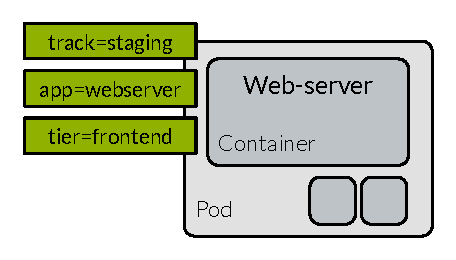
\includegraphics[width=7cm]{figures/kubernetes/labels}
    \caption{Labels}
    \label{fig:labels_report}
\end{figure}

\noindent
The second bad lesson learned in running Borg is \textbf{One IP address per machine complicates things}. \textit{"In Borg, all tasks on a machine use the single IP address of their host, and thus share the host's port space"}  \cite[p. 14]{verma2015borg}. This results in port allocation management because of a limited number ports. Kubernetes solves this problem by leveraging software-defined networking that allows every pod to get its own IP address. This allows \textit{"developers to choose ports rather than requiring their software to adapt to the ones chosen by the infrastructure and removes the infrastructure complexity of managing ports"} \cite[p. 13]{verma2015borg}. \\


\noindent
Other important concepts in Kubernetes are \textit{replica sets} and \textit{deployments}. A replica set ensures that a specified number of pods "replicas" are running at any given time. Replica sets are a lower level concept that is not controlled directly, instead replica sets are controlled through a deployment. Figure~\ref{fig:replica_sets_report} shows an example with three pods and a replica set managed by a deployment. Users can specify any given desired number of replicas wanted. The replica set will work towards the desired state, and keep it. If a node suddenly is removed, all pods running on this node will be rescheduled to a new node, and the desired number of replicas will be maintained.

\begin{figure}[H]
    \centering
    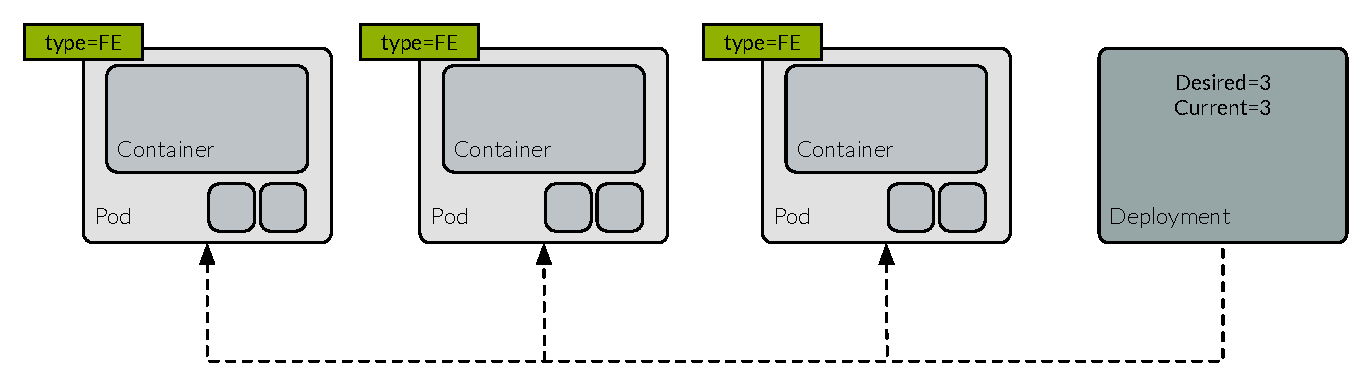
\includegraphics[width=15cm]{figures/kubernetes/replica_sets}
    \caption{Replica Sets}
    \label{fig:replica_sets_report}
\end{figure}

\noindent
A deployment is, as mentioned, a higher-level concept that manages replica sets, pods and provides declarative updates to pods along with a lot of other useful features \cite{kubernetesio}. It is only necessary to describe the desired state in a deployment object, and the deployment controller will then change the actual state to the desired state at a controlled rate. Deployments can be described in a declarative manner using YAML files leveraging the ideas of \textit{infrastructure as code\footnote{\url{http://martinfowler.com/bliki/InfrastructureAsCode.html}}}. The deployment of a new version is done in a controlled manner at a controlled rate. One pod will be replaced at a time with the new version until all of the replicas are replaced with a new pod.